\documentclass[assign]{article}

\usepackage{graphicx}
\usepackage{amsmath,amssymb,amsthm} % define this before the line numbering.
\usepackage{color}
\usepackage{eso-pic}
\usepackage{bm}
\usepackage{caption}
\usepackage{microtype}
\usepackage{epstopdf}
\usepackage{picins}
\usepackage[boxed]{algorithm2e}

% Declaring commonly used math operators
\DeclareMathOperator{\ddiag}{Diag}
\DeclareMathOperator{\rrank}{rank}
\DeclareMathOperator{\vvec}{vec}
\DeclareMathOperator{\tr}{tr}

\newcommand{\PhiB}{\mathbf{\Phi}}
\newcommand{\Ll}{\mathcal{L}}
\newcommand{\Nn}{\mathcal{N}}
\newcommand{\Uu}{\mathcal{U}}
\newcommand{\Ee}{\mathcal{E}}
\newcommand{\Aa}{\mathcal{A}}
\newcommand{\Hh}{\mathcal{H}}
\newcommand{\Ii}{\mathcal{I}}
\newcommand{\Ff}{\mathcal{F}}
\newcommand{\Dd}{\mathcal{D}}
\newcommand{\Tt}{\mathcal{T}}
\newcommand{\Pp}{\mathcal{P}}
\newcommand{\Ss}{\mathcal{S}}
\newcommand{\Cc}{\mathcal{C}}
\newcommand{\Bb}{\mathcal{B}}
\newcommand{\Rr}{\mathcal{R}}
\newcommand{\Rm}{\mathrm{R}}
\newcommand{\CB}{\mathbf{C}}
\newcommand{\RB}{\mathbf{R}}
\newcommand{\xB}{\mathbf{x}}
\newcommand{\yB}{\mathbf{y}}
\newcommand{\fB}{\mathbf{f}}
\newcommand{\ZB}{\mathbf{Z}}
\newcommand{\SB}{\mathbf{S}}
\newcommand{\AB}{\mathbf{A}}
\newcommand{\WB}{\mathbf{W}}
\newcommand{\TB}{\mathbf{T}}

\newcommand{\omitme}[1]{}
\newtheorem*{lemma}{Lemma}
\newtheorem{case}{Case}

\title{Homework 2}

\author{Prateep Mukherjee}

\begin{document}
\maketitle

\noindent 1. a)  The maximum contiguous subarray problem can be solved using a dynamic programming algorithm as follows:

\begin{algorithm}[!hbt]
%  \SetAlgoLined
 % \DontPrintSemicolon
  \caption{Maximum contiguous subarray sum}
  \KwIn{$A$ : array of numbers, which may be positive, negative, or zero}
  \KwOut{maximum sum of elements in a contiguous subarray $A[i \ldots j]$}
%  \KwProc{blah}
  \tcp{Initialize global and local maximum sums}
  $res \gets 0$\; 
  $current\_max \gets 0$\;
   \For{$i = 1 \ldots n$} {
        \uIf{$current\_max + A_i > current\_max$ } {
              \tcp{Add $A_i$ to $current\_max$ if it improves later}
              $current\_max \gets current\_max + A_i$\;
        }  \Else { \tcp{Begin a new subarray at $i$} 
           $current\_max \gets A_i$\; \label{line1}
        }
        \tcp{Update global maximum if $current\_max$ improves former}
        \If {$current\_max > res$} {
             $res \gets current\_max$\;
         }        
   }
   \KwRet{res}
\label{algo3}
\end{algorithm}

Complexity of Algorithm \ref{algo3} is $\Theta(n)$, as we are iterating over the array just once. 

\textbf{Proof of Correctness:}  Let, $S$ be the current maximum in subarray ending at index $j$ ($j < n$). Now, we add $A_{j+1}$ to $S$, if it increases $S$. This means, we can get a larger sum, ending at $j+1$, by including $A_{j+1}$ to our current maximum. 
The above condition is possible only when $A_{j+1} > 0$. Hence, in the case when $A_{j+1} < 0$, we begin a new subarray starting at index $j+1$. 

\textbf {A special case in this problem, is when all the elements of $A$ are negative.} In such a scenario, we argue that our algorithm produces the correct result, which is the maximum of all the elements in $A$. In this case, each $A_i$ will decrease the value of $current\_max$. So, for each element, the algorithm will go to else condition and update $current\_max$. The global maximum $res$, then will be equal to the maximum element in the array.

\noindent (b) The maximum contiguous array product problem is solved using a similar approach as in (a). One observation here, however, is that if an element of $A$ is negative, a current minimum negative product can be multiplied with it to get the largest positive product. Hence, we need two running maximum positive and minimum negative products. The algorithm can be written as follows:

\begin{algorithm}
%  \SetAlgoLined
%  \DontPrintSemicolon
  \caption{Maximum contiguous array product}
  \KwIn{$A$ : array of integers, which may be both positive or negative or zero}
  \KwOut{Maximum product in a contiguous subarray of A}
  $res \gets 1$\;
  $maxpos \gets 1$ \tcp{Maximum running positive product $\ge 1$}
  $minneg \gets 1$ \tcp{Minimum running negative product $\le 1$}
 
  \For{$i = 1 \ldots n$} {
       \uIf{$A_i > 0$} {
           \tcp{Update $maxpos$ over here.$minneg$ will be updated if $minneg < 0$, in which case it will get smaller}
            $maxpos \gets maxpos \times A_i$\;
            $minneg \gets \min{(minneg \times A_i, 1)}$\;
        } \uElseIf {$A_i < 0$} {
           \tcp{If $minneg < 0$, $maxpos$ will be updated, else $maxpos = 1$.$minneg$ will be updated to last $maxpos \times A_i$. }
            $prev \gets maxpos$\;
            $maxpos \gets \max{(minneg \times A_i,1)}$\;
            $minneg \gets prev \times A_i$\;
        } \Else {
           \tcp{Begin new subarray at $i$}
           $maxpos \gets 1$\;
           $minneg \gets 1$\;
        }

       \tcp{Update global maximum if $maxpos$ improves former}
        \If{$maxpos > res$} {
             $res \gets maxpos$ \;
         }
  } 
  \KwRet{res}
  \label{algo4}
\end{algorithm}
\vspace{-10pt}

Complexity of algorithm \ref{algo4} is $\Theta(n)$ as we are iterating over the array only once.

\noindent \textbf{Proof of Correctness:} As seen in Algorithm \ref{algo4}, we have two variables, storing maximum positive and minimum negative products. Now, if $A_i > 0$, we simply update the maximum positive product. This is done in the first {\em if} in Algorithm \ref{algo4} However, if $A_i < 0$, we can get an even bigger product than $maxpos$ by multiplying the minimum negative product and $A_i$. The minimum negative product, using similar analogy, will be the product of the previous $maxpos$ and $A_i$. This is done in {\em else if} condition. Finally, we cannot include $A_i = 0$ elements in our result. Hence, we begin a new subarray if we see a $A_i = 0$. This is the {\em else} check.

\vspace{10pt}

\noindent 2. The given problem can be solved using a dynamic programming algorithm. However, first we need to pre-process the input string to generate the number of palindromes at each element of the string. Let, $L[i][j]$ denote the number of palindromes of length $j$ ending at $S_i$. This can be generated in $\Theta(n^2)$ time complexity by checking the number of palindromes of length 1, 2 and so on, with the end character being $S_i$. 

\noindent The subproblem of the DP solution is as follows. $L[i][j]$ is updated only when there is at least one palindrome of length $j-2$ ending at $S_{i-1}$. Thus, pseudo-code for computing $L[i][j]$ for the entire string $S$ can be written as:

\begin{algorithm}[H]
%  \SetAlgoLined
%  \DontPrintSemicolon
   \caption{{\sc Preprocess:} Compute $L$}
  \tcp{Each character in $S$ is a palindrome in itself.} 
  $L[i][0] = 1 $\;
   \For{$i \gets 0 \ldots \left | S\right |$} {
        \For{$j \gets 2 \ldots \left | S\right |$} {
              \tcp{Check if there is at least one palindrome of length $j-2$ ending at $S_{i-1}$}
              \uIf{$j == 2 $}  { \tcp{Two characters, hence a palindrome} 
                  $L[i][j] = 1$\;  
               } \Else { \tcp{Check maximum length palindrome ending at $S_{i-1}$}
                   $len \gets \left | L[i-1] \right|$\;
		     \tcp{If there exists palindrome of length $j-2$ ending at $S_{i-1}$, we add to our list a palindrome of length $j$ ending at $S_i$ }
                   \If{$L[i-1][len] == j-2$} {
                          $L[i][j] = 1$;
                    }
               }
         }
    }
\end{algorithm}

\noindent Having generated $L$, we can now use dynamic programming to generate an optimal result. Let, $A[i]$ denote the minimum number of palindromes in $S[0 \ldots i-1]$. Then,

\vspace{-10pt}
\begin{equation}
    A[i+1] = \min{(A[i-L[i][j]] + 1, \forall j \in [0 \ldots \left | L[i] \right |] )} 
\label{eq1}
\end{equation}

\noindent Solving eq. \ref{eq1} is also $\Theta(n^2)$ time complexity. Overall time complexity of this algorithm is thus $\Theta(n^2)$.

\noindent \textbf{Proof of correctness:} $L_{ij}$ stores the number of palindromes of length $j$ with the last character in the palindrome being $S_i$. Now, $A_i$ will have the minimum number of palindromes in the substring $S[0 \cdots i-1]$. $A_i$ is computed taking the minimum of all palindromes ending at $S_{i-1}$. Therefore, $A_i$ must have the minimum number of palindromes in the substring $S[0 \cdots i-1]$. Finally, $A_{|S|}$ gives us the required result.

\vspace{10pt}

\noindent 3.  The first obvious algorithm that one might use to solve this problem is greedy-based - choose the exit nearest to the current location with the maximum capacity to drop-off students, reach that exit traveling forward or backward, drop students off at that exit and repeat the algorithm until there is at least one student left in the bus. However, this algorithm does not give us the optimal solution. 

\piccaption{ \label{greedy} \small The red circles show the exits, with the one pointed by an arrow being the current location. The numbers in black are the time required to travel between the exits, and those in green represent the maximum number of students that can be dropped at each exit.
}
\parpic[r] {
\begin{minipage}{0.5\textwidth}
{
  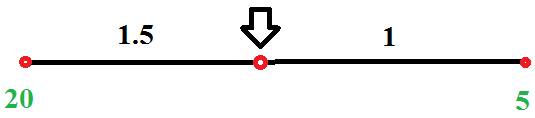
\includegraphics[width=\linewidth] {3_1.png}
  \vspace{-3pt}
}
\end{minipage}
}

In Fig.\ref{greedy}, we see an example of the greedy algorithm. Let the initial number of students in the bus be 20. Using the greedy algorithm, we will choose the exit on the right, drop 5 students over there and come back to the original location. Thus, the total 
amount of soda that will be consumed is $20 \times 1 + 15 \times 1 = 35.$  However, if we chose the right direction, the maximum amount of soda consumed will be $20 \times 1.5 = 30.$ This simple example proves that a greedy algorithm will not give the optimal strategy.

\noindent The other option is to use a dynamic programming method. The first observation we make is that visited exits on the highway should be contiguous. This means that we can go to an exit not yet visited, only from either its immediate left visited or right visited exit. 


So, given a state of visited exits, we can only make two possible transitions - go to the immediate left unvisited exit, or the immediate right unvisited one. The optimal solution solution, of course, is the minimum of them. It is to be noted here that at \textbf{each transition we are decreasing the number of unvisited exits by one}. Hence, our algorithm is guarranted to converge.   

\noindent Now, let us define the state of our DP solution. Let, $<lhs, rhs, dir>$ denote the left and right-hand side exits which are yet not visited, given that every exit $\{ e | lhs < e < rhs\}$ has been visited before, and $dir$ is a boolean variable denoting which direction the bus is travelling. The DP recurrence relation can now be written as follows:

\vspace{-10pt}
\begin{eqnarray}
   <lhs, rhs, dir> = \min\left\{ \begin{array} {cc}
        <lhs + 1, rhs, dir = true>, \\
        <lhs, rhs - 1, dir = false>
 \end{array} \right\}  
\label{eq2}
\end{eqnarray}

\noindent The base case of our algorithm is when $lhs + 1 == rhs$, which we can compute using the time it takes to travel from exit $lhs$ to $rhs$. Solving eq.\ref{eq2} naively will lead us to an exponential time algorithm, as to solve each problem we are computing twice as many subproblems. This is solved by using {\em memoization} technique, or caching the previously computed interval results. Eq. \ref{eq2} can be implemented using a 2D array of all exits, where each cell $(i,j)$ denote the state $<i,j,dir>$. The array is computed using $\Theta (n^2)$, where $n$ is the total number of exits. 

\noindent \textbf{Proof of Correctness:} To solve each subproblem, we are taking the minimum time of two transitions, traversing left and right. This has to be the optimal way of traversal, as we have to travel contiguous exits.  

\vspace{10pt}

\noindent 4. a) The naive approach to compute the minimum number of bills to make {\emph k} Dream Dollars is to try all possible combinations of the given denominations. The algorithm proceeds as follows:

\begin{algorithm}[H]
% \SetAlgoLined
 % \DontPrintSemicolon
 \caption{Solve\_Naive}
 \SetKwFunction{solve}{solve}
 \KwIn{coin denominations $C = \{ c_1, c_2, c_3, \ldots c_n \}$, {\emph K} }
 \KwOut{Minimum number of coins, from given denominations, to generate {\emph K} Dream Dollars}
 $best \gets -1$\; 
 $numCoinsSoFar \gets 0$\;
 
 $\solve(C, {\emph K} )$ { \\
 \For{$c \in C$} {
    $change \gets {\emph K} - c$\; 
    \If{ $change > 0 \quad || \quad numCoinsSoFar +1 \ge best$} {
       \uIf{$change = 0$} {
          $best \gets numCoinsSoFar + 1$\;
       } \Else {
          $numCoinsSoFar = numCoinsSoFar + 1$\;
          \BlankLine
          $\solve(C,change)$\;            
          \BlankLine
          $numCoinsSoFar = numCoinsSoFar - 1$\;
       }
    }
  }
  }
  \KwRet{best}
  \label{algo1}
\end{algorithm}


Algorithm \ref{algo1} includes each denomination once and recomputes the entire procedure using the change($> 0$). The complexity of the algorithm is $\Theta \left( 2^{\emph{K} }\right)$.

\noindent \textbf{Proof of Correctness:} The naive approach covers the entire search space of possible solutions, and chooses the minimum one. Hence, it always generates the optimal solution. 


b) The dynamic programming algorithm proceeds as follows. Let, $S$ be an array, where every element $S_j$ represents the minimum number of coins to generate $j$ Dream Dollars. $S$ is initialized to 0. 

The algorithm can be stated simply as follows. For each coin $c$, $c \le k$, look at the minimum number of coins found for the $k-c$ Dream Dollars(which we have found previously). Let, this number be $p$. If $p+1$ is less than the minimum number of coins already found for the current sum $k$, then we update $S_k$.

The Pseudo-code for this algorithm can be written as:

\begin{algorithm}[H]
% \SetAlgoLined
%  \DontPrintSemicolon
  \caption{Solve\_DP}
  \KwIn{Dream Dollar \emph{K}}
  \KwOut{Minimum number of coins, from given denominations, to generate {\emph K} Dream Dollars}
   $S[0 \ldots MAX] \gets \infty$ \tcp{MAX is the maximum possible Dream Dollar amount} 
   
   \For{$k = 1 \ldots K$} {
     \For{$c \in C$} {
        \If{$c \le k \quad \& \quad S[k-c]+1 < S[k]$} {
             $S[k] \gets S[k-c] + 1$\;
        }
     }
   } 
  \KwRet{$S[\emph{K}]$} 
\label{algo2}
\end{algorithm}


Algorithm \ref{algo2} computes current value in $S$ based on previously computed numbers. Complexity of 
the above algorithm is $\Theta \left( \emph{K}\left| C \right|\right)$. 

\textbf{Proof Of Correctness} At each step of algorithm \ref{algo2} we update our current answer for denomination $k$ if and only if we find a better answer using a coin of lesser denomination. Therefore, at each step we are computing the optimal result for denomination $k$.

(c) (i) Table \ref{tab1} shows the runtimes of naive and DP algorithms for a set of dream dollars. The denominations used are $\{ 1, 4, 7, 13, 28, 52, 91, 365\}$. The results for naive and DP methods matched in each of the cases.


 \begin{table}[!hbt]
   \caption{Computation time(in seconds) for different denominations.}
   \vspace{-10pt}
   \begin{center}
    \begin{tabular}{| c | c | c |}
      \hline
       Denomination & Naive & DP \\
      \hline
       10 & 0.18 & 0.10 \\
      \hline
       15 & 0.04 & 0.12 \\ 
      \hline
       20 & 0.12 & 0.12 \\
      \hline
       25 & 0.21 & 0.13 \\ 
       \hline
       30 & 0.26 & 0.14 \\
      \hline
       35 & 0.33 & 0.15 \\ 
       \hline
       40 & 0.47 & 0.19 \\
      \hline
       45 & 0.70 & 0.20 \\ 
      \hline
       50 & 1.00 & 0.19 \\
      \hline
       55 & 0.74 & 0.21 \\
      \hline
    \end{tabular}       
   \end{center}
   \label{tab1}
\end{table}  

(ii) In this section, we report the difference in results from greedy and dynamic programming algorithms.

\begin{table}[!hbt]
  \caption{Minimum number of coins as reported by Greedy \& DP algorithms}
\vspace{-10pt}
  \begin{center}
    \begin{tabular}{| c | c | c |}
       \hline
       {\emph K} & Greedy & DP \\
       \hline
       416 & 7 & 5 \\
       \hline
       455 & 7 & 5 \\
       \hline 
       507 & 8 & 6 \\
       \hline 
       546 & 8 & 6 \\
       \hline 
       598 & 9 & 7 \\
       \hline
    \end{tabular}
  \end{center}
  \label{tab2}
\end{table}


It is obvious from Table \ref{tab2} that the greedy algorithm fails to report the optimal result in many cases. Let, $proc$ denote the procedure name for coin exchange problem. For example, for $\emph{K} = 416$, the greedy algorithm works as follows.

\vspace{-10pt}
\begin{equation}
  proc(416) \equiv \{ 1 (\$ \; 365) , 1 (\$ \; 28) , 1 (\$ \; 13) , 1(\$ \; 7) , 3(\$ \; 1) \} \equiv {7} \notag
\end{equation}

The DP method, however, finds an optimal solution as follows.

\begin{equation}
  proc(416) \equiv \{ 4 (\$ \; 91) , 1 (\$ \; 52) \} \equiv {5} \notag
\end{equation}


%\begin{equation}
%   \tilde{p}(x_i) \approx \frac{1}{M} \sum_{j=1, j\neq i}^{M} G(\textcolor{red}{f_i}\frac{\xB_i - \xB_j}{k_j}, \sigma_i)
%\end{equation}

\end{document}
